
\begin{frame}[fragile,label=L7second]{The Exceptional Seven Element Lattice}
  \begin{center}
    {\scalefont{.75}
      \begin{tikzpicture}[scale=.7]
              \node (J1) at (0,1)  [draw, circle, inner sep=\dotsize] {};
      \draw (.36, 1) node {$J_1$};
      \node (H) at (1,0)  [draw, circle, inner sep=\dotsize] {};
      \draw (1.16, -.2) node {$H$};
      \node (M2) at (1,2)  [draw, circle, inner sep=\dotsize] {};
      \draw (1.4, 2) node {$M_2$};
      \node (J2) at (2,1)  [draw, circle, inner sep=\dotsize] {};
      \draw (2.2, .8) node {$J_2$};
      \node (G) at (2,3)  [draw, circle, inner sep=\dotsize] {};
      \draw (2.3, 3.1) node {$G$};
      \node (M1) at (3,2)  [draw, circle, inner sep=\dotsize] {};
      \draw (3.35, 2) node {$M_1$};
      \node (K) at (-1,1.2)  [draw, circle, inner sep=\dotsize] {};
      \draw (-1.28, 1.15) node {$K$};

      \draw[semithick] (H) to (J1) to (M2) to (G) to (M1) to (J2) to (H) (J2) to (M2);
      \draw[semithick] (H) to (K) to (G);

      \end{tikzpicture}
    }
  \end{center}

\begin{theorem}
\label{thm:except-seven-elem}
Suppose $H<G$, $\core_G(H) = 1$, and 
$L_7 \cong [H,G]$.  Then
\begin{enumerate}[(i)]
\item<1-> $G$ is a primitive permutation group.
\item<1-> If $N\ssubnormal G$, then $C_G(N) = 1$.
\item<1-> $G$ contains no non-trivial abelian normal subgroup.
\item<1-> $G$ is not solvable.
\item<1-> $G$ is subdirectly irreducible.
\item<1-> With the possible exception of at most one maximal subgroup, $M_1$ or $M_2$,
  all proper subgroups in the interval $[H,G]$ are core-free. 

%% The three subgroups in $[H,G]$ which cover $H$ (the atoms) are
%%   core-free.  At least one two of the three maximal subgroups (the co-atoms) in
%%   the interval are core-free. 
\end{enumerate}
\end{theorem}
%% \note{  It is obvious that 
%%   \begin{itemize}
%%   \item (ii) $\Rightarrow$ (iii) $\Rightarrow$ (iv), and  
%% \item (ii) $\Rightarrow$ (v), but we include these for
%%   emphasis;
%% \item the hard work is in proving (ii) and (vi), but
%%   the main goal is the pair of restrictions (iii) and (v), which allow us to rule
%%   out a number of the O'Nan-Scott types describing primitive permutation
%%   groups. 
%%   \end{itemize}}
\end{frame}

\begin{frame}[fragile,label=IdeaOfL7Proof]{Idea of the proof}
    %% \begin{column}{0.3\textwidth}
      \begin{center}
        {\scalefont{.78}
          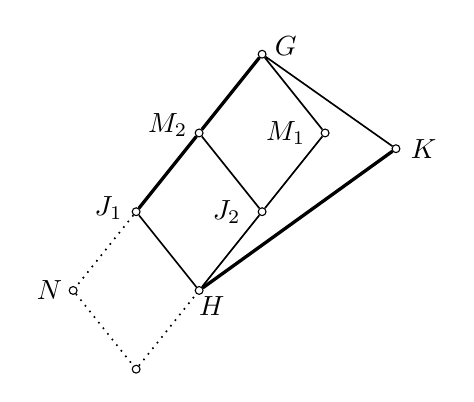
\begin{tikzpicture}[scale=1]
      \node (N) at (-.6,0)  [draw, circle, inner sep=1pt] {};
      \draw (-.9, 0) node {$N$};
      \node (NcapH) at (.2,-1)  [draw, circle, inner sep=1pt] {};
      \node (J1) at (0.2,1)  [draw, circle, inner sep=1pt] {};
      \draw (-.15, 1.05) node {$J_1$};
      \node (H) at (1,0)  [draw, circle, inner sep=1pt] {};
      \draw (1.16, -.2) node {$H$};
      \node (M2) at (1,2)  [draw, circle, inner sep=1pt] {};
      \draw (.6, 2.1) node {$M_2$};
      \node (J2) at (1.8,1)  [draw, circle, inner sep=1pt] {};
      \draw (1.35, 1.) node {$J_2$};
      \node (G) at (1.8,3)  [draw, circle, inner sep=1pt] {};
      \draw (2.1, 3.1) node {$G$};
      \node (M1) at (2.6,2)  [draw, circle, inner sep=1pt] {};
      \draw (2.1, 2) node {$M_1$};
      \node (K) at (3.5,1.8)  [draw, circle, inner sep=1pt] {};
      \draw (3.85, 1.8) node {$K$};
      \draw[semithick,dotted] (J1) to (N) to (NcapH) to (H);
      \visible<4->{\draw[very thick] (J1) to (M2) to (G) (H) to (K);}
      \draw[semithick] (J1) to (M2) to (G) (H) to (K);
      \draw[semithick] (H) to (J1) to (M2) to (G) to (M1) to (J2) to (H) to (K)
      to (G) (J2) to (M2);
    \end{tikzpicture}
 }
\end{center}
      
  %%   \end{column}
  %% \end{columns}

  %% \begin{columns}
  %%   \begin{column}{0.7\textwidth}
      {\bf Claim:} 
      $J_1$ and $J_2$ are core-free subgroups of $G$.\\[6pt]
      {\bf Proof:}
      \begin{itemize}
      \item<2->
      If $N\ssubnormal G$ then $NH$ permutes with each subgroup containing $H$.  
      \note{Let $H \leq X \leq G$.  Then $NHX = NX = XN= XHN = XNH$.}
      \item<3-> If $1\neq N\leq J_1$, then $NH = J_1$, so $J_1$ and $K$ permute.
      \item<4-> Since $J_1K = G$ and $J_1\cap K = H$, our lemma yields
      \[
        [J_1, G] \cong [H, K]^{J_1} = \{X \in[H, K] \mid J_1X=XJ_1 \}.
        \]
   \uncover<5->{Impossible!}
      \end{itemize}

    %% \end{column}


\end{frame}

\begin{frame}[fragile,label=OSTheorem]{Achbacher-O'Nan-Scott Theorem}
Let $G$ be a primitive permutation
group of degree $d$, and let $N := \Soc(G) \cong T^m$ with $m \geq 1$. 
Then one of the following holds.
\vskip2mm
\begin{enumerate}
\item 
$N$ is regular and
  \begin{itemize}
  \item 
  \alert{Affine type} $T$ is cyclic of order $p$, so $|N| = p^m$ . Then 
$d = p^m$ and $G$ is permutation isomorphic to a subgroup of the affine
general linear group $\AGL(m,p)$.
\vskip2mm
\item \alert{Twisted wreath product type} $m \geq 6$, the group $T$ is 
  nonabelian and $G$ is a group of \emph{twisted wreath product type}, with
  $d = |T|^m$.
  \end{itemize}
\vskip2mm
\item $N$ is non-regular, non-abelian, and
  \begin{itemize}
  \item 
\alert{Almost simple} $m = 1$ and $T \leq G \leq \Aut(T)$.
\vskip2mm
\item \alert{Product action} $m \geq 2$ and $G$ is permutation isomorphic to a
subgroup of the product action wreath product $P \wr S_{m/l}$ of degree
$d = nm/l$. The group $P$ is primitive of type 2.(a) or 2.(c), $P$ has
degree $n$ and $\Soc(P) \cong T^l$, where $l \geq 1$ divides $m$.
\vskip2mm
\item 
\alert{Diagonal type} $m \geq 2$ and $T^m \leq G \leq T^m . (\Out(T ) \times S_m)$, with
the diagonal action. The degree $d = |T|^{m-1}$.
  \end{itemize}
\end{enumerate}
\end{frame}

